% 编译：xelatex paper_with_figures_main.tex
% 在 docs 目录下执行，以便正确找到 figures/ 下的图片
% 若您已有主文档，只需将本文件中的“五、实验与结果”部分
% （即 % ============================================================
% 五、实验设置与结果（插入到主文档 \section*{四、...} 之后）
% 使用方式：在主 .tex 中 % ============================================================
% 五、实验设置与结果（插入到主文档 \section*{四、...} 之后）
% 使用方式：在主 .tex 中 % ============================================================
% 五、实验设置与结果（插入到主文档 \section*{四、...} 之后）
% 使用方式：在主 .tex 中 \input{paper_section_experiments} 或直接粘贴本段
% 图表文件：将以下 4 张图放入与主 .tex 同级的 figures/ 目录：
%   - train_loss_curve.png   （训练损失曲线）
%   - length_curve.png       （生成长度 vs 参考长度）
%   - structure_coverage.png  （四段结构覆盖率）
%   - grade_confusion.png    （分类混淆矩阵）
% ============================================================

\section*{五、实验设置与结果（Experiments and Results）}

\subsection*{5.1 实验设置}

\textbf{数据与任务：} 采用私有肺结节 CT 影像-报告配对数据及 pGGN 浸润分级标注（AAH/AIS/MIA/IAC 四分类）；训练阶段使用 Stage~2 联合优化“描述生成 + 分级诊断”，视觉编码保留 28$\times$28 级别高分辨率特征，Mamba-2.8B 作为语言骨干。

\textbf{训练配置：} 最大视觉 token 数 144，最大文本长度 640，batch size 4，学习率 1e-5，epoch 30；梯度裁剪与梯度累积按需启用；日志与 checkpoint 落盘至指定输出目录。

\textbf{验证与评测：} 在 23 例私有验证集上运行端到端推理（报告生成 + 结节勾画 + 分级预测），从 \texttt{meta.json} 与逐样本输出中汇总：报告四段结构通过率、幻觉率、生成长度分布、结节勾画成功率、分类准确率及混淆矩阵。

\subsection*{5.2 主要数值结果}

表~\ref{tab:exp-summary} 给出本次验证 run（run\_20260228\_192037）的汇总指标，供正文引用。

\begin{table}[htbp]
\centering
\footnotesize
\renewcommand{\arraystretch}{1.2}
\begin{tabular}{ll}
\toprule
\textbf{指标} & \textbf{数值} \\
\midrule
验证样本数 & 23 \\
报告四段结构通过率 & 0.00\% \\
幻觉率（规则检测） & 30.43\% \\
生成长度均值 / 中位数 & 215.9 / 210 \\
参考长度均值 / 中位数 & 427.2 / 356 \\
结节勾画成功率 & 100\% \\
分级可评估样本数 & 16 \\
分级分类准确率 & 100\% \\
\bottomrule
\end{tabular}
\caption{私有验证 run\_20260228\_192037 汇总指标（summary.json）。}
\label{tab:exp-summary}
\end{table}

\subsection*{5.3 附图（可直接放汇报/论文）}

\textbf{图~\ref{fig:train-loss}：训练损失曲线。} Stage~2 训练过程中 caption loss 随 step 变化，用于说明收敛情况。

% 插入位置 1：训练损失曲线
\begin{figure}[htbp]
\centering
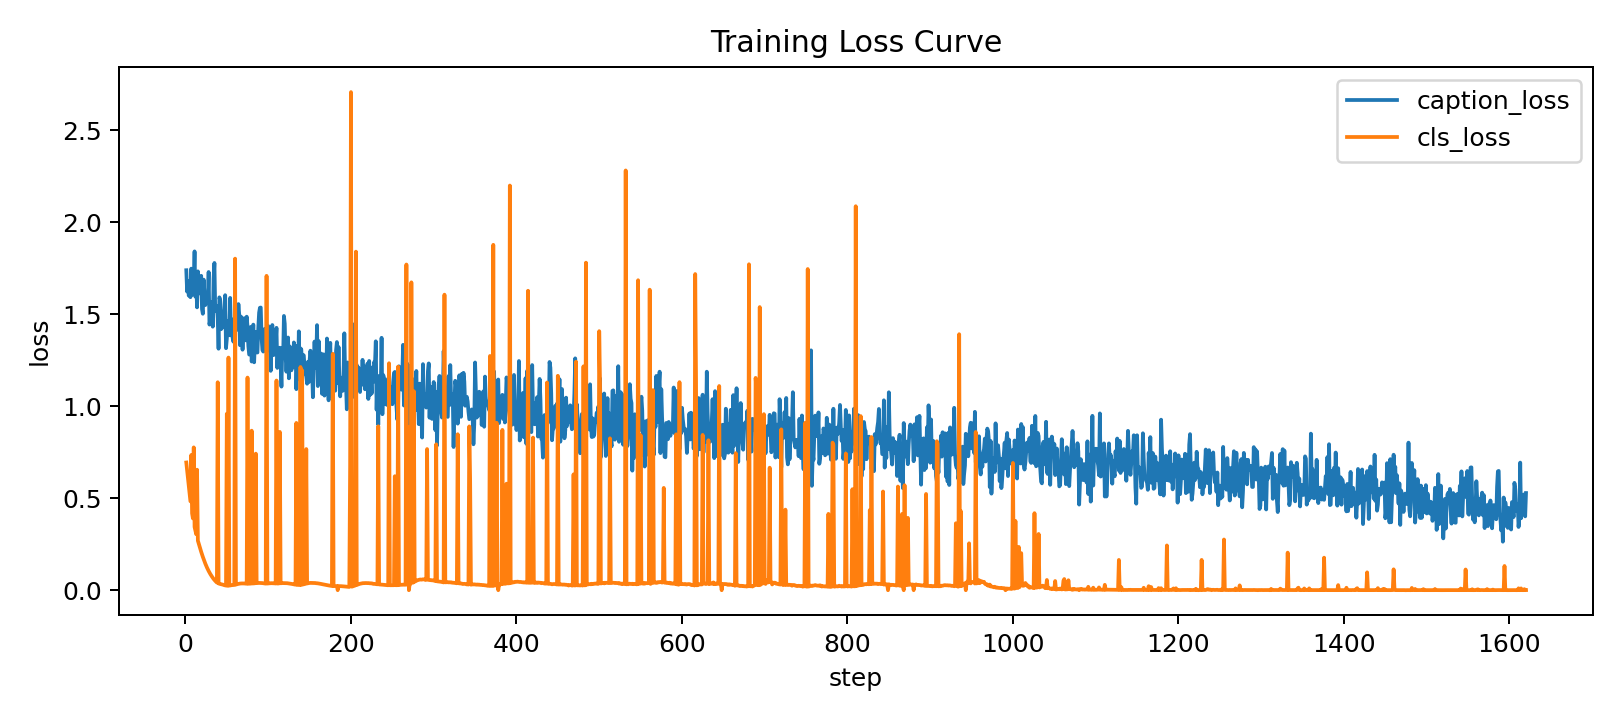
\includegraphics[width=0.85\linewidth]{figures/train_loss_curve}
\caption{Stage~2 训练损失曲线（caption loss vs.\ training step）。}
\label{fig:train-loss}
\end{figure}

\textbf{图~\ref{fig:length-curve}：生成长度 vs.\ 参考长度。} 生成报告 token 长度与参考报告长度的分布对比，用于分析文本长度与截断情况。

% 插入位置 2：生成长度 vs 参考长度
\begin{figure}[htbp]
\centering
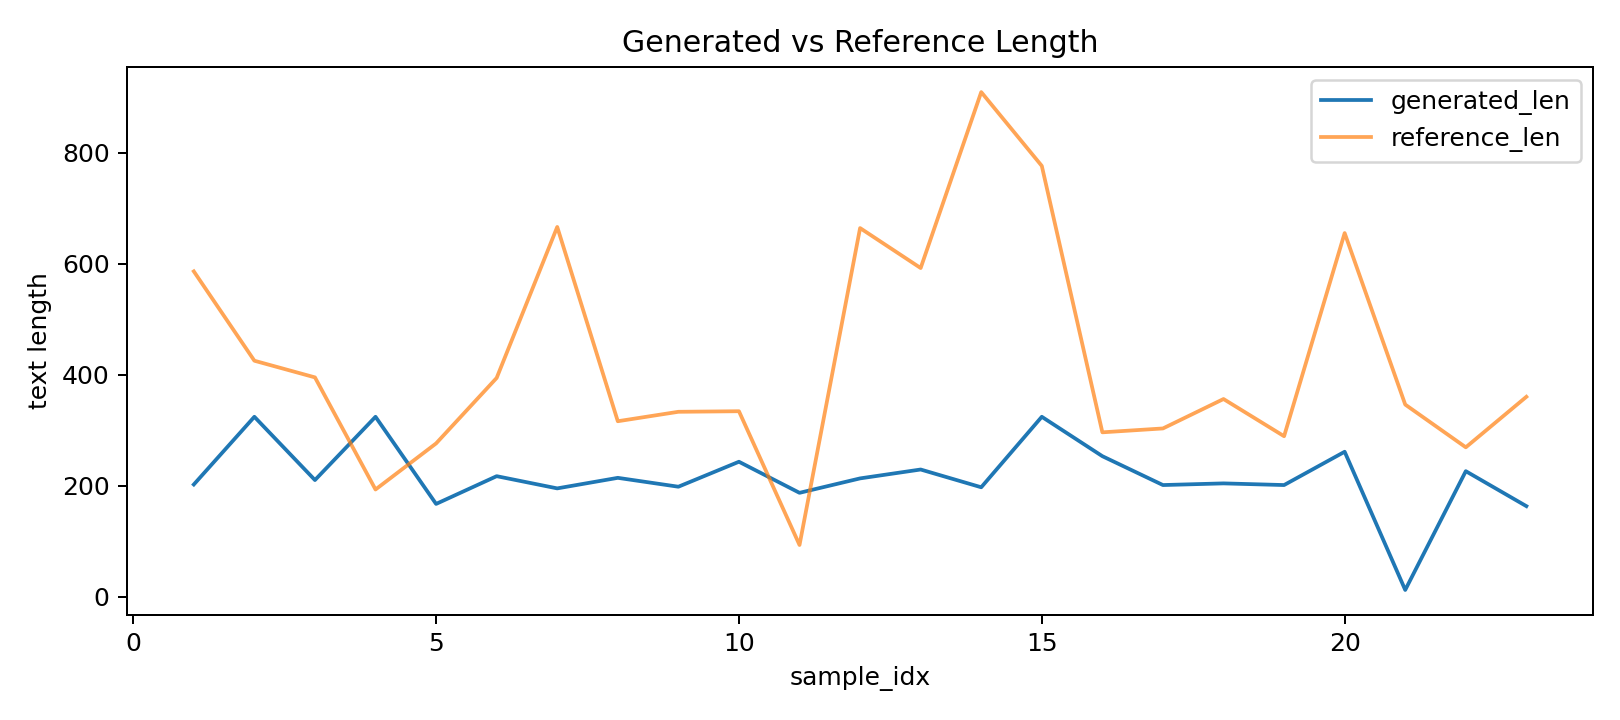
\includegraphics[width=0.85\linewidth]{figures/length_curve}
\caption{生成长度与参考长度分布（length\_curve）。}
\label{fig:length-curve}
\end{figure}

\textbf{图~\ref{fig:structure-coverage}：四段结构覆盖率。} 报告“所见 / 结论 / 建议 / 病理倾向”四段结构的覆盖情况。

% 插入位置 3：四段结构覆盖率
\begin{figure}[htbp]
\centering
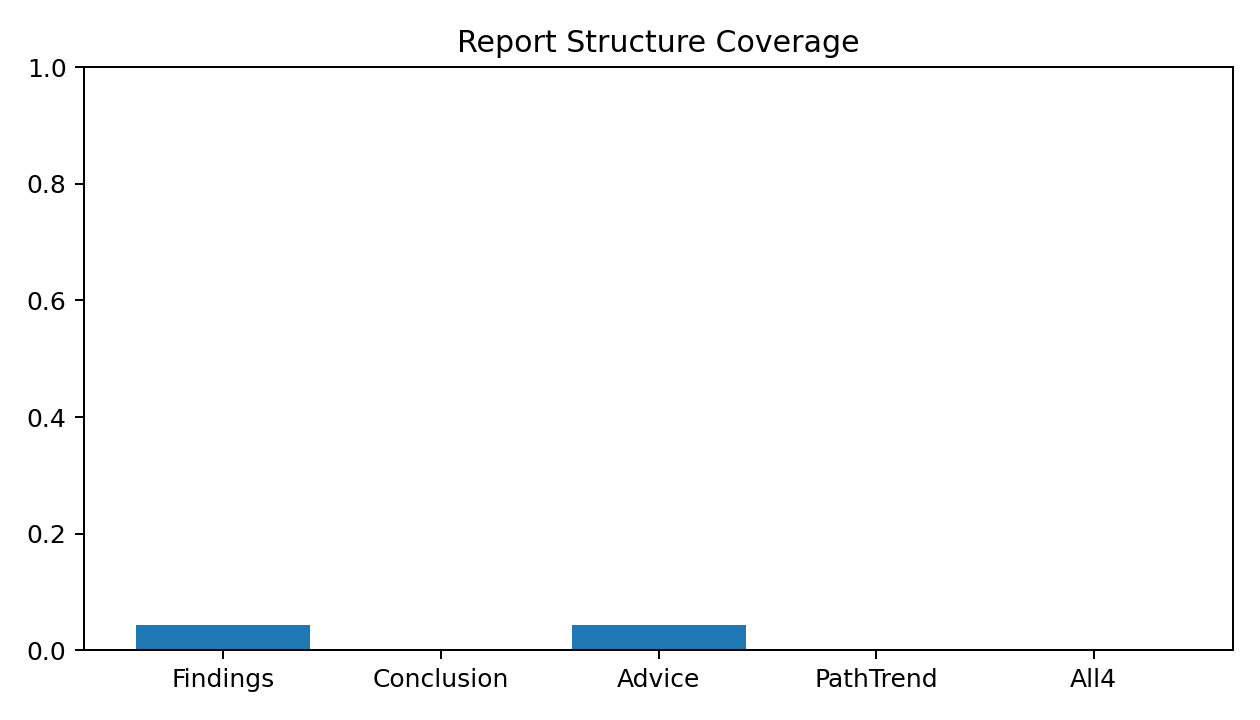
\includegraphics[width=0.85\linewidth]{figures/structure_coverage}
\caption{四段结构覆盖率（structure\_coverage）。}
\label{fig:structure-coverage}
\end{figure}

\textbf{图~\ref{fig:grade-confusion}：分类混淆矩阵。} 浸润等级（AAH/AIS/MIA/IAC）预测与真实标签的混淆矩阵。

% 插入位置 4：分类混淆矩阵
\begin{figure}[htbp]
\centering
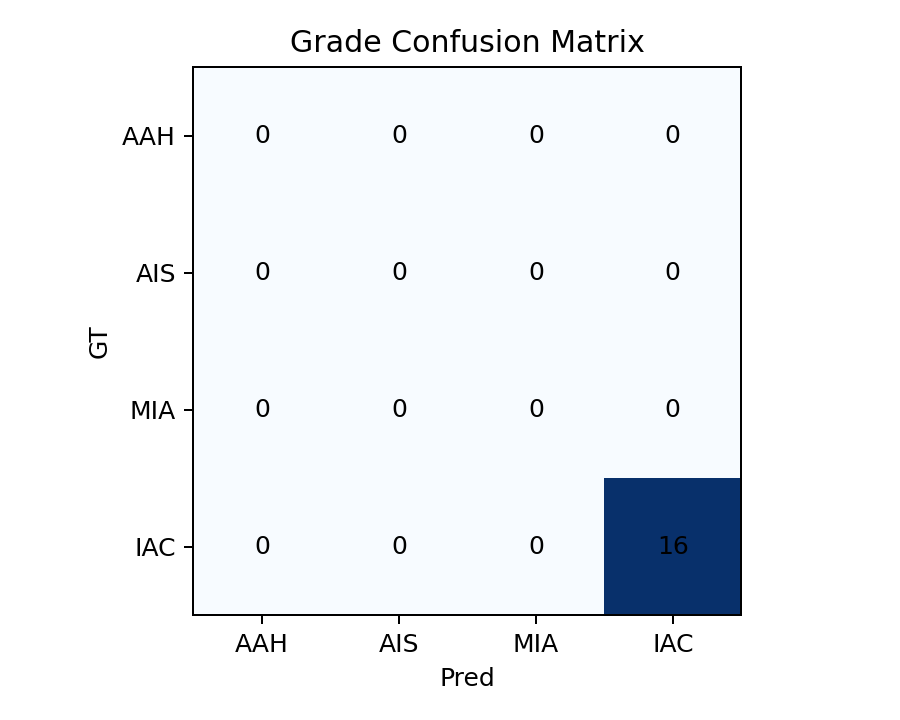
\includegraphics[width=0.75\linewidth]{figures/grade_confusion}
\caption{浸润等级分类混淆矩阵（grade\_confusion）。}
\label{fig:grade-confusion}
\end{figure}

\subsection*{5.4 小结}

上述结果来自单次验证 run，表明：在现有私有数据与设定下，结节勾画与分级分类可达较高成功率；报告四段通过率与幻觉率仍有优化空间，建议结合约束解码与模板检查进一步改进（见 EXPERIMENT\_REPORT.md 中的建议）。训练损失曲线与结构/长度/混淆矩阵图可直接用于方法章节或附录的“实验与结果”部分。
 或直接粘贴本段
% 图表文件：将以下 4 张图放入与主 .tex 同级的 figures/ 目录：
%   - train_loss_curve.png   （训练损失曲线）
%   - length_curve.png       （生成长度 vs 参考长度）
%   - structure_coverage.png  （四段结构覆盖率）
%   - grade_confusion.png    （分类混淆矩阵）
% ============================================================

\section*{五、实验设置与结果（Experiments and Results）}

\subsection*{5.1 实验设置}

\textbf{数据与任务：} 采用私有肺结节 CT 影像-报告配对数据及 pGGN 浸润分级标注（AAH/AIS/MIA/IAC 四分类）；训练阶段使用 Stage~2 联合优化“描述生成 + 分级诊断”，视觉编码保留 28$\times$28 级别高分辨率特征，Mamba-2.8B 作为语言骨干。

\textbf{训练配置：} 最大视觉 token 数 144，最大文本长度 640，batch size 4，学习率 1e-5，epoch 30；梯度裁剪与梯度累积按需启用；日志与 checkpoint 落盘至指定输出目录。

\textbf{验证与评测：} 在 23 例私有验证集上运行端到端推理（报告生成 + 结节勾画 + 分级预测），从 \texttt{meta.json} 与逐样本输出中汇总：报告四段结构通过率、幻觉率、生成长度分布、结节勾画成功率、分类准确率及混淆矩阵。

\subsection*{5.2 主要数值结果}

表~\ref{tab:exp-summary} 给出本次验证 run（run\_20260228\_192037）的汇总指标，供正文引用。

\begin{table}[htbp]
\centering
\footnotesize
\renewcommand{\arraystretch}{1.2}
\begin{tabular}{ll}
\toprule
\textbf{指标} & \textbf{数值} \\
\midrule
验证样本数 & 23 \\
报告四段结构通过率 & 0.00\% \\
幻觉率（规则检测） & 30.43\% \\
生成长度均值 / 中位数 & 215.9 / 210 \\
参考长度均值 / 中位数 & 427.2 / 356 \\
结节勾画成功率 & 100\% \\
分级可评估样本数 & 16 \\
分级分类准确率 & 100\% \\
\bottomrule
\end{tabular}
\caption{私有验证 run\_20260228\_192037 汇总指标（summary.json）。}
\label{tab:exp-summary}
\end{table}

\subsection*{5.3 附图（可直接放汇报/论文）}

\textbf{图~\ref{fig:train-loss}：训练损失曲线。} Stage~2 训练过程中 caption loss 随 step 变化，用于说明收敛情况。

% 插入位置 1：训练损失曲线
\begin{figure}[htbp]
\centering
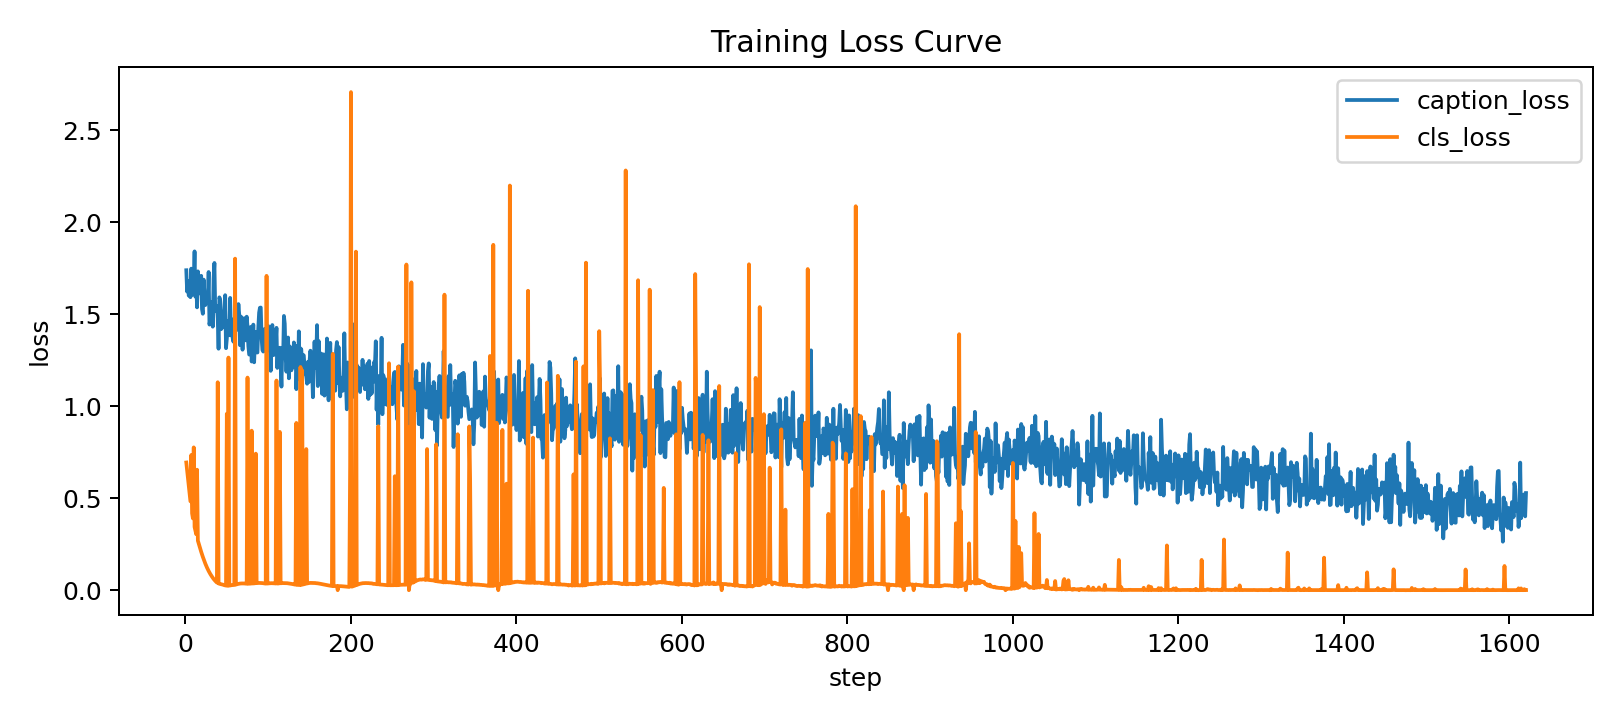
\includegraphics[width=0.85\linewidth]{figures/train_loss_curve}
\caption{Stage~2 训练损失曲线（caption loss vs.\ training step）。}
\label{fig:train-loss}
\end{figure}

\textbf{图~\ref{fig:length-curve}：生成长度 vs.\ 参考长度。} 生成报告 token 长度与参考报告长度的分布对比，用于分析文本长度与截断情况。

% 插入位置 2：生成长度 vs 参考长度
\begin{figure}[htbp]
\centering
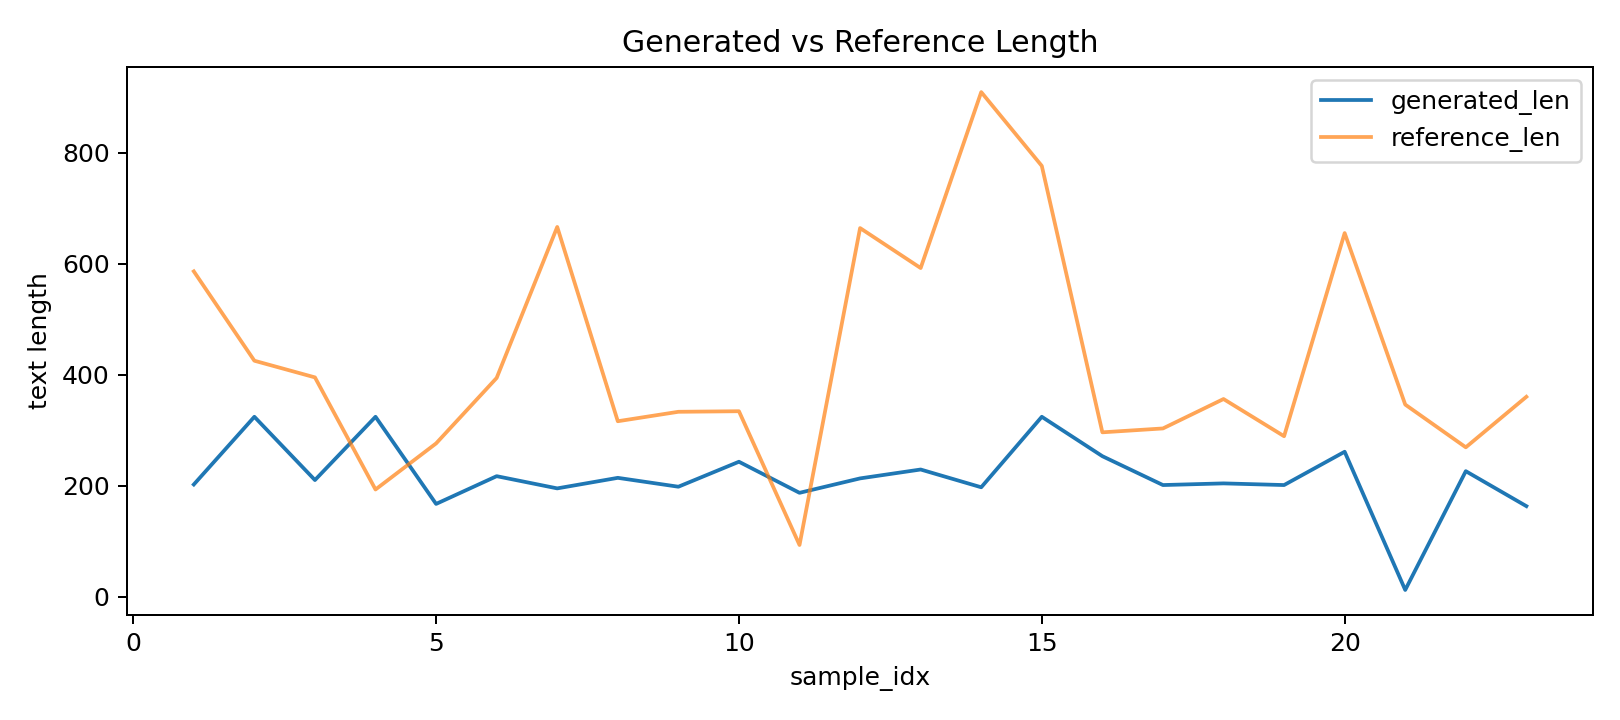
\includegraphics[width=0.85\linewidth]{figures/length_curve}
\caption{生成长度与参考长度分布（length\_curve）。}
\label{fig:length-curve}
\end{figure}

\textbf{图~\ref{fig:structure-coverage}：四段结构覆盖率。} 报告“所见 / 结论 / 建议 / 病理倾向”四段结构的覆盖情况。

% 插入位置 3：四段结构覆盖率
\begin{figure}[htbp]
\centering
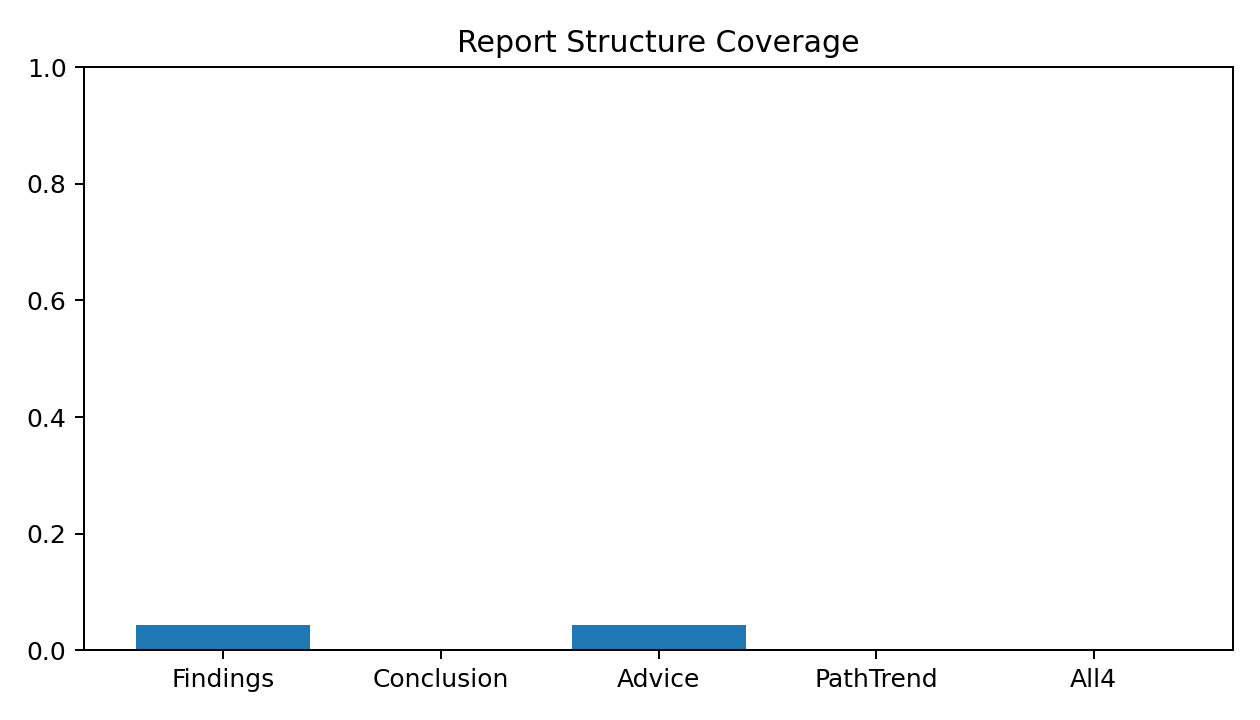
\includegraphics[width=0.85\linewidth]{figures/structure_coverage}
\caption{四段结构覆盖率（structure\_coverage）。}
\label{fig:structure-coverage}
\end{figure}

\textbf{图~\ref{fig:grade-confusion}：分类混淆矩阵。} 浸润等级（AAH/AIS/MIA/IAC）预测与真实标签的混淆矩阵。

% 插入位置 4：分类混淆矩阵
\begin{figure}[htbp]
\centering
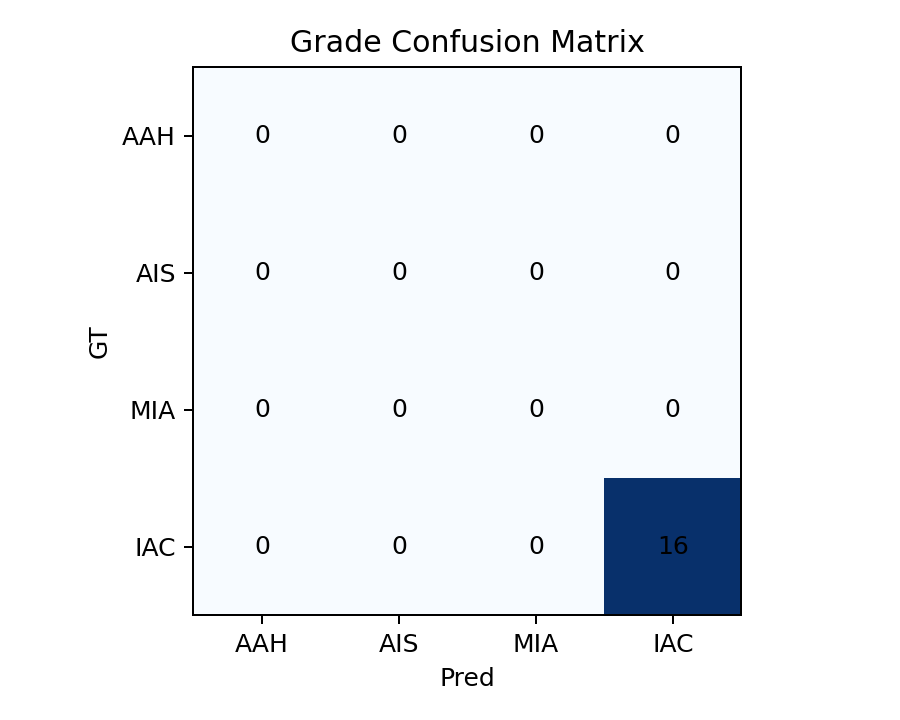
\includegraphics[width=0.75\linewidth]{figures/grade_confusion}
\caption{浸润等级分类混淆矩阵（grade\_confusion）。}
\label{fig:grade-confusion}
\end{figure}

\subsection*{5.4 小结}

上述结果来自单次验证 run，表明：在现有私有数据与设定下，结节勾画与分级分类可达较高成功率；报告四段通过率与幻觉率仍有优化空间，建议结合约束解码与模板检查进一步改进（见 EXPERIMENT\_REPORT.md 中的建议）。训练损失曲线与结构/长度/混淆矩阵图可直接用于方法章节或附录的“实验与结果”部分。
 或直接粘贴本段
% 图表文件：将以下 4 张图放入与主 .tex 同级的 figures/ 目录：
%   - train_loss_curve.png   （训练损失曲线）
%   - length_curve.png       （生成长度 vs 参考长度）
%   - structure_coverage.png  （四段结构覆盖率）
%   - grade_confusion.png    （分类混淆矩阵）
% ============================================================

\section*{五、实验设置与结果（Experiments and Results）}

\subsection*{5.1 实验设置}

\textbf{数据与任务：} 采用私有肺结节 CT 影像-报告配对数据及 pGGN 浸润分级标注（AAH/AIS/MIA/IAC 四分类）；训练阶段使用 Stage~2 联合优化“描述生成 + 分级诊断”，视觉编码保留 28$\times$28 级别高分辨率特征，Mamba-2.8B 作为语言骨干。

\textbf{训练配置：} 最大视觉 token 数 144，最大文本长度 640，batch size 4，学习率 1e-5，epoch 30；梯度裁剪与梯度累积按需启用；日志与 checkpoint 落盘至指定输出目录。

\textbf{验证与评测：} 在 23 例私有验证集上运行端到端推理（报告生成 + 结节勾画 + 分级预测），从 \texttt{meta.json} 与逐样本输出中汇总：报告四段结构通过率、幻觉率、生成长度分布、结节勾画成功率、分类准确率及混淆矩阵。

\subsection*{5.2 主要数值结果}

表~\ref{tab:exp-summary} 给出本次验证 run（run\_20260228\_192037）的汇总指标，供正文引用。

\begin{table}[htbp]
\centering
\footnotesize
\renewcommand{\arraystretch}{1.2}
\begin{tabular}{ll}
\toprule
\textbf{指标} & \textbf{数值} \\
\midrule
验证样本数 & 23 \\
报告四段结构通过率 & 0.00\% \\
幻觉率（规则检测） & 30.43\% \\
生成长度均值 / 中位数 & 215.9 / 210 \\
参考长度均值 / 中位数 & 427.2 / 356 \\
结节勾画成功率 & 100\% \\
分级可评估样本数 & 16 \\
分级分类准确率 & 100\% \\
\bottomrule
\end{tabular}
\caption{私有验证 run\_20260228\_192037 汇总指标（summary.json）。}
\label{tab:exp-summary}
\end{table}

\subsection*{5.3 附图（可直接放汇报/论文）}

\textbf{图~\ref{fig:train-loss}：训练损失曲线。} Stage~2 训练过程中 caption loss 随 step 变化，用于说明收敛情况。

% 插入位置 1：训练损失曲线
\begin{figure}[htbp]
\centering
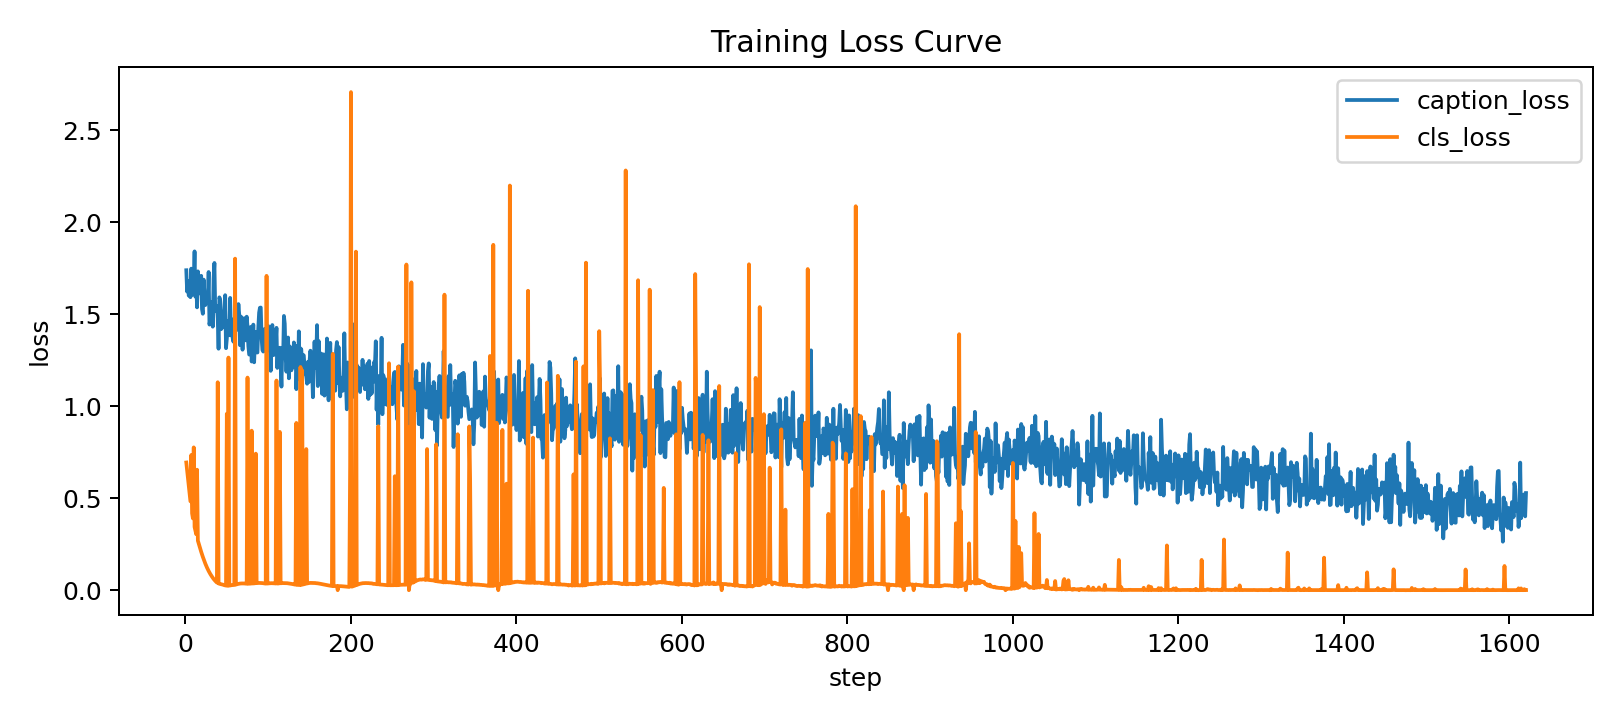
\includegraphics[width=0.85\linewidth]{figures/train_loss_curve}
\caption{Stage~2 训练损失曲线（caption loss vs.\ training step）。}
\label{fig:train-loss}
\end{figure}

\textbf{图~\ref{fig:length-curve}：生成长度 vs.\ 参考长度。} 生成报告 token 长度与参考报告长度的分布对比，用于分析文本长度与截断情况。

% 插入位置 2：生成长度 vs 参考长度
\begin{figure}[htbp]
\centering
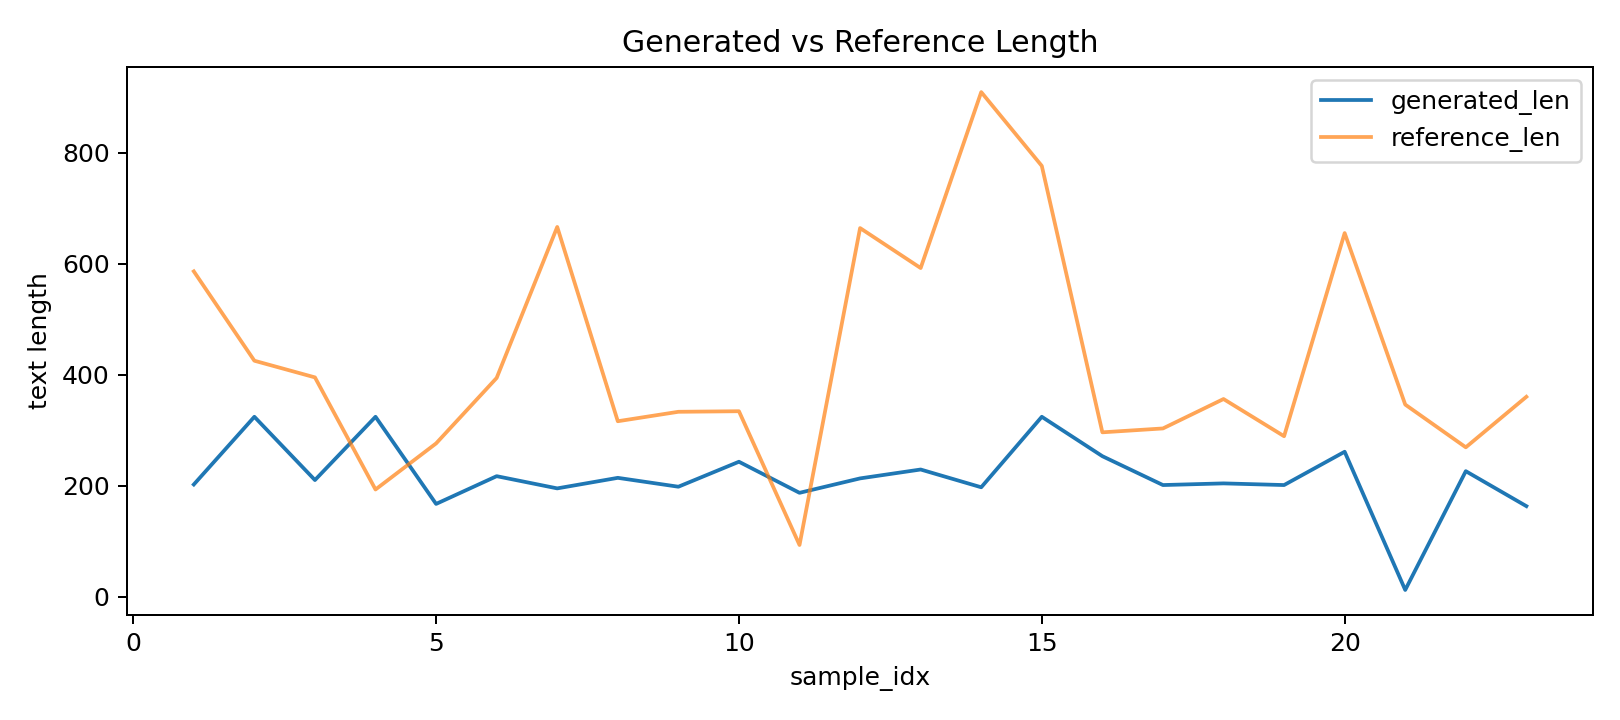
\includegraphics[width=0.85\linewidth]{figures/length_curve}
\caption{生成长度与参考长度分布（length\_curve）。}
\label{fig:length-curve}
\end{figure}

\textbf{图~\ref{fig:structure-coverage}：四段结构覆盖率。} 报告“所见 / 结论 / 建议 / 病理倾向”四段结构的覆盖情况。

% 插入位置 3：四段结构覆盖率
\begin{figure}[htbp]
\centering
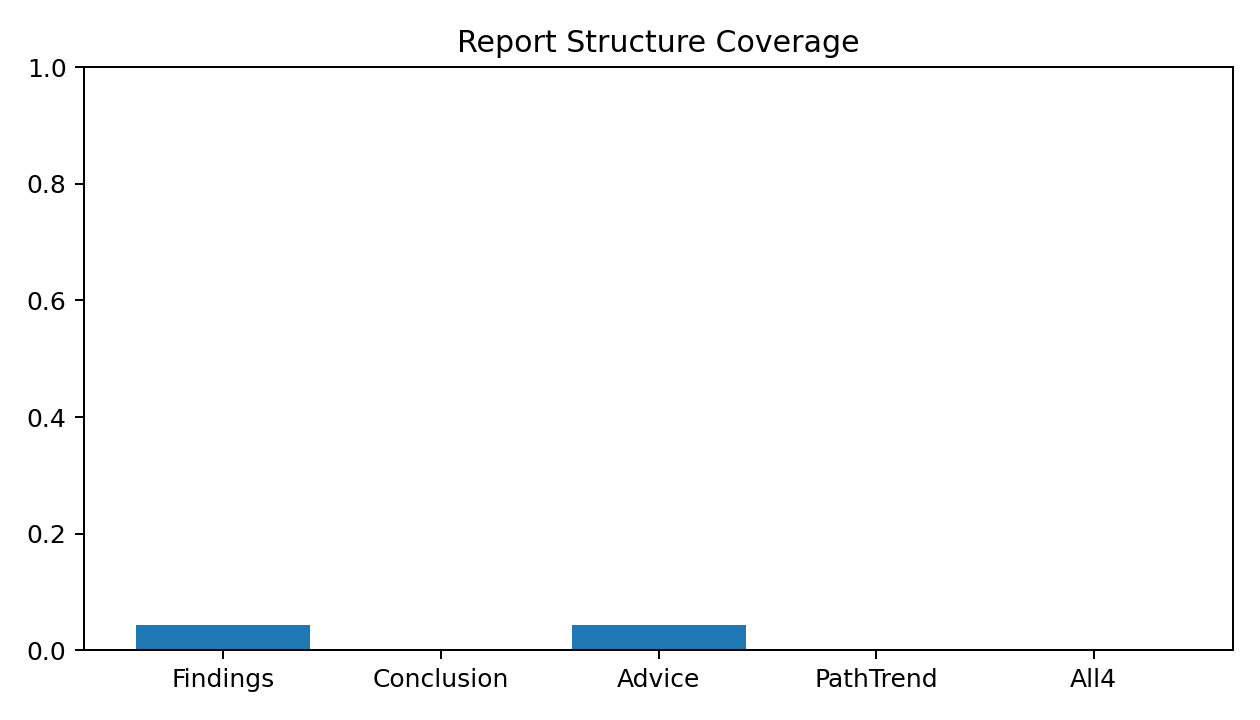
\includegraphics[width=0.85\linewidth]{figures/structure_coverage}
\caption{四段结构覆盖率（structure\_coverage）。}
\label{fig:structure-coverage}
\end{figure}

\textbf{图~\ref{fig:grade-confusion}：分类混淆矩阵。} 浸润等级（AAH/AIS/MIA/IAC）预测与真实标签的混淆矩阵。

% 插入位置 4：分类混淆矩阵
\begin{figure}[htbp]
\centering
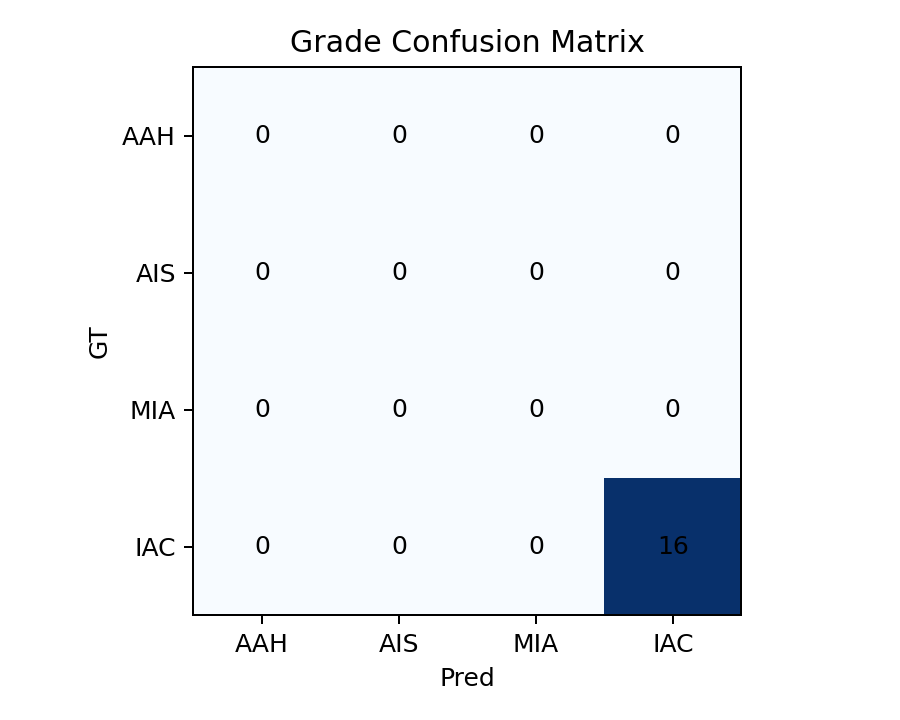
\includegraphics[width=0.75\linewidth]{figures/grade_confusion}
\caption{浸润等级分类混淆矩阵（grade\_confusion）。}
\label{fig:grade-confusion}
\end{figure}

\subsection*{5.4 小结}

上述结果来自单次验证 run，表明：在现有私有数据与设定下，结节勾画与分级分类可达较高成功率；报告四段通过率与幻觉率仍有优化空间，建议结合约束解码与模板检查进一步改进（见 EXPERIMENT\_REPORT.md 中的建议）。训练损失曲线与结构/长度/混淆矩阵图可直接用于方法章节或附录的“实验与结果”部分。
 或该 section 的完整内容）
% 插入到您主文档中“四、针对已有工作的改进与对比实验建议”之后、参考文献之前。
\documentclass[11pt]{article}
\usepackage[UTF8,scheme=plain,fontset=none]{ctex}
\usepackage[margin=1in]{geometry}
\usepackage{amsmath}
\usepackage{graphicx}
\usepackage{booktabs}
\usepackage{tabularx}
\usepackage{array}
\usepackage{hyperref}
\hypersetup{colorlinks=true,linkcolor=blue,urlcolor=blue,citecolor=blue}
\setlength{\parindent}{0pt}

\begin{document}

\section*{四、针对已有工作的改进与对比实验建议}
（此处保留您原文“四、……”的完整内容；此处仅占位。）

\clearpage
% ========== 图表插入位置：下方为“五、实验设置与结果” ==========
% ============================================================
% 五、实验设置与结果（插入到主文档 \section*{四、...} 之后）
% 使用方式：在主 .tex 中 % ============================================================
% 五、实验设置与结果（插入到主文档 \section*{四、...} 之后）
% 使用方式：在主 .tex 中 % ============================================================
% 五、实验设置与结果（插入到主文档 \section*{四、...} 之后）
% 使用方式：在主 .tex 中 \input{paper_section_experiments} 或直接粘贴本段
% 图表文件：将以下 4 张图放入与主 .tex 同级的 figures/ 目录：
%   - train_loss_curve.png   （训练损失曲线）
%   - length_curve.png       （生成长度 vs 参考长度）
%   - structure_coverage.png  （四段结构覆盖率）
%   - grade_confusion.png    （分类混淆矩阵）
% ============================================================

\section*{五、实验设置与结果（Experiments and Results）}

\subsection*{5.1 实验设置}

\textbf{数据与任务：} 采用私有肺结节 CT 影像-报告配对数据及 pGGN 浸润分级标注（AAH/AIS/MIA/IAC 四分类）；训练阶段使用 Stage~2 联合优化“描述生成 + 分级诊断”，视觉编码保留 28$\times$28 级别高分辨率特征，Mamba-2.8B 作为语言骨干。

\textbf{训练配置：} 最大视觉 token 数 144，最大文本长度 640，batch size 4，学习率 1e-5，epoch 30；梯度裁剪与梯度累积按需启用；日志与 checkpoint 落盘至指定输出目录。

\textbf{验证与评测：} 在 23 例私有验证集上运行端到端推理（报告生成 + 结节勾画 + 分级预测），从 \texttt{meta.json} 与逐样本输出中汇总：报告四段结构通过率、幻觉率、生成长度分布、结节勾画成功率、分类准确率及混淆矩阵。

\subsection*{5.2 主要数值结果}

表~\ref{tab:exp-summary} 给出本次验证 run（run\_20260228\_192037）的汇总指标，供正文引用。

\begin{table}[htbp]
\centering
\footnotesize
\renewcommand{\arraystretch}{1.2}
\begin{tabular}{ll}
\toprule
\textbf{指标} & \textbf{数值} \\
\midrule
验证样本数 & 23 \\
报告四段结构通过率 & 0.00\% \\
幻觉率（规则检测） & 30.43\% \\
生成长度均值 / 中位数 & 215.9 / 210 \\
参考长度均值 / 中位数 & 427.2 / 356 \\
结节勾画成功率 & 100\% \\
分级可评估样本数 & 16 \\
分级分类准确率 & 100\% \\
\bottomrule
\end{tabular}
\caption{私有验证 run\_20260228\_192037 汇总指标（summary.json）。}
\label{tab:exp-summary}
\end{table}

\subsection*{5.3 附图（可直接放汇报/论文）}

\textbf{图~\ref{fig:train-loss}：训练损失曲线。} Stage~2 训练过程中 caption loss 随 step 变化，用于说明收敛情况。

% 插入位置 1：训练损失曲线
\begin{figure}[htbp]
\centering
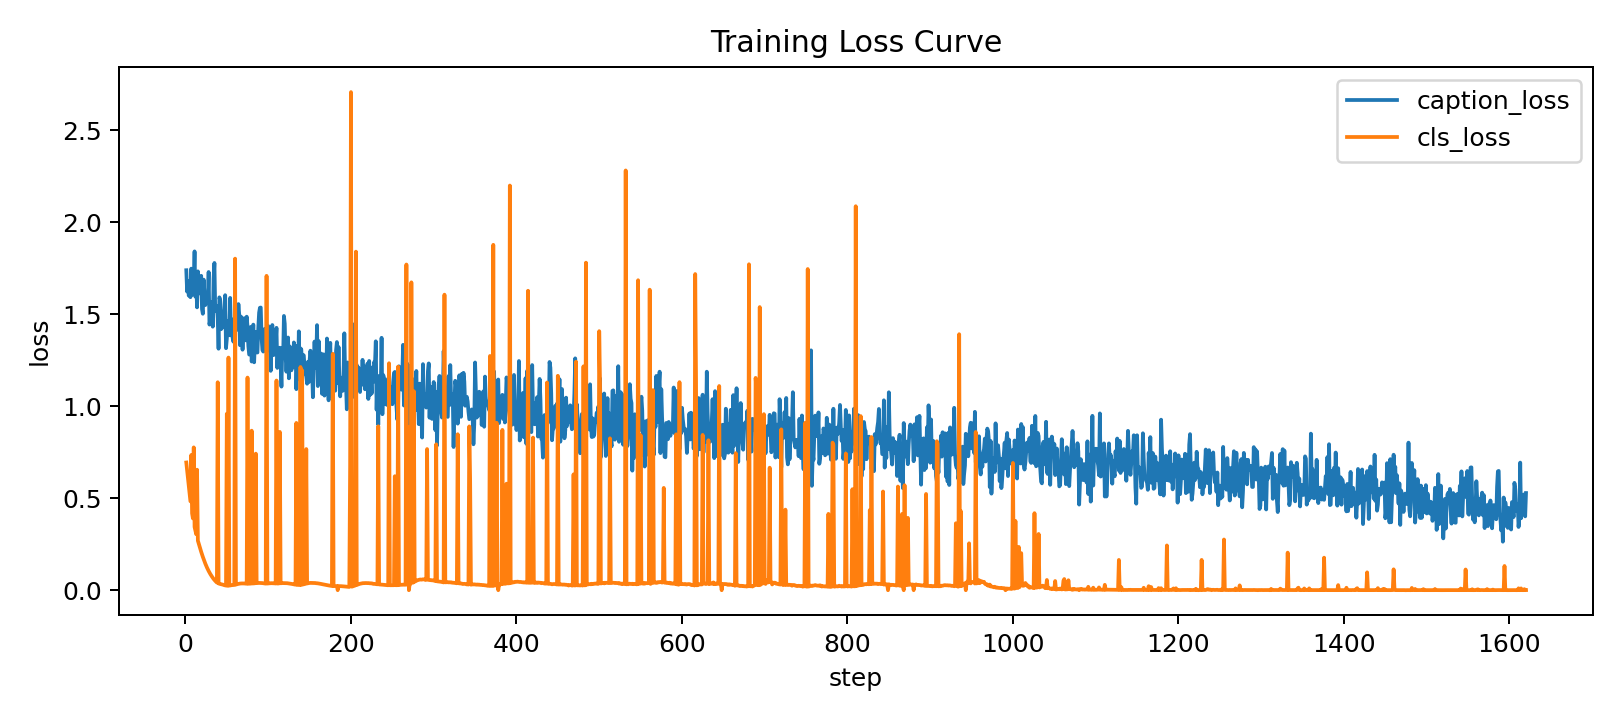
\includegraphics[width=0.85\linewidth]{figures/train_loss_curve}
\caption{Stage~2 训练损失曲线（caption loss vs.\ training step）。}
\label{fig:train-loss}
\end{figure}

\textbf{图~\ref{fig:length-curve}：生成长度 vs.\ 参考长度。} 生成报告 token 长度与参考报告长度的分布对比，用于分析文本长度与截断情况。

% 插入位置 2：生成长度 vs 参考长度
\begin{figure}[htbp]
\centering
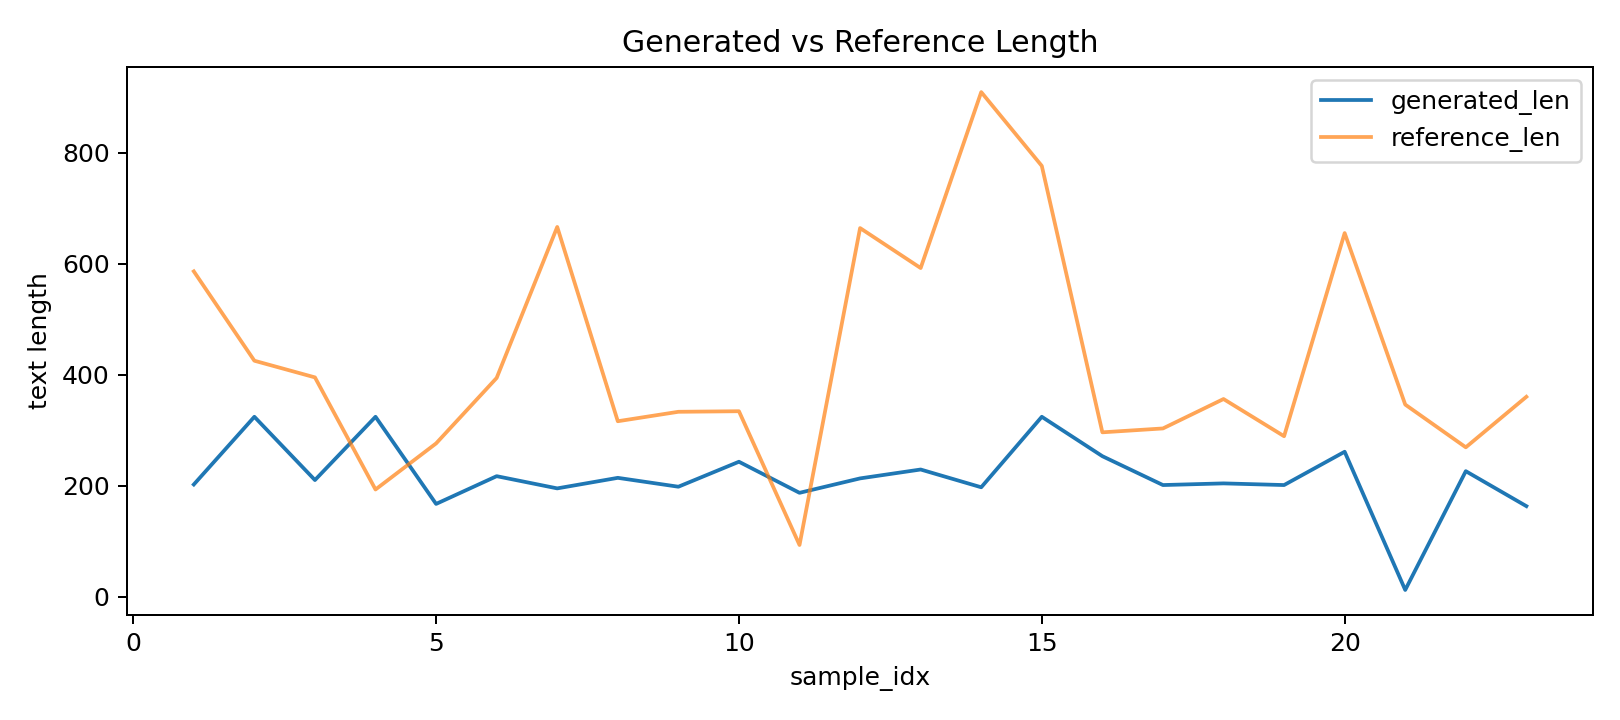
\includegraphics[width=0.85\linewidth]{figures/length_curve}
\caption{生成长度与参考长度分布（length\_curve）。}
\label{fig:length-curve}
\end{figure}

\textbf{图~\ref{fig:structure-coverage}：四段结构覆盖率。} 报告“所见 / 结论 / 建议 / 病理倾向”四段结构的覆盖情况。

% 插入位置 3：四段结构覆盖率
\begin{figure}[htbp]
\centering
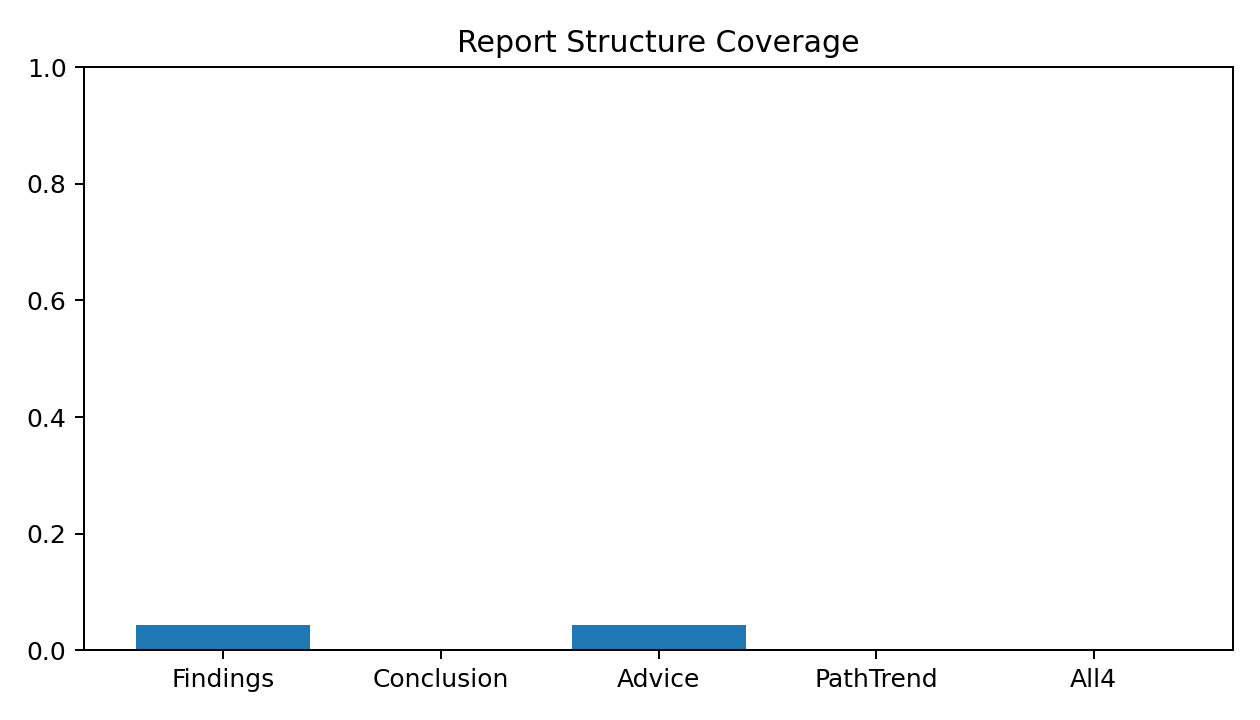
\includegraphics[width=0.85\linewidth]{figures/structure_coverage}
\caption{四段结构覆盖率（structure\_coverage）。}
\label{fig:structure-coverage}
\end{figure}

\textbf{图~\ref{fig:grade-confusion}：分类混淆矩阵。} 浸润等级（AAH/AIS/MIA/IAC）预测与真实标签的混淆矩阵。

% 插入位置 4：分类混淆矩阵
\begin{figure}[htbp]
\centering
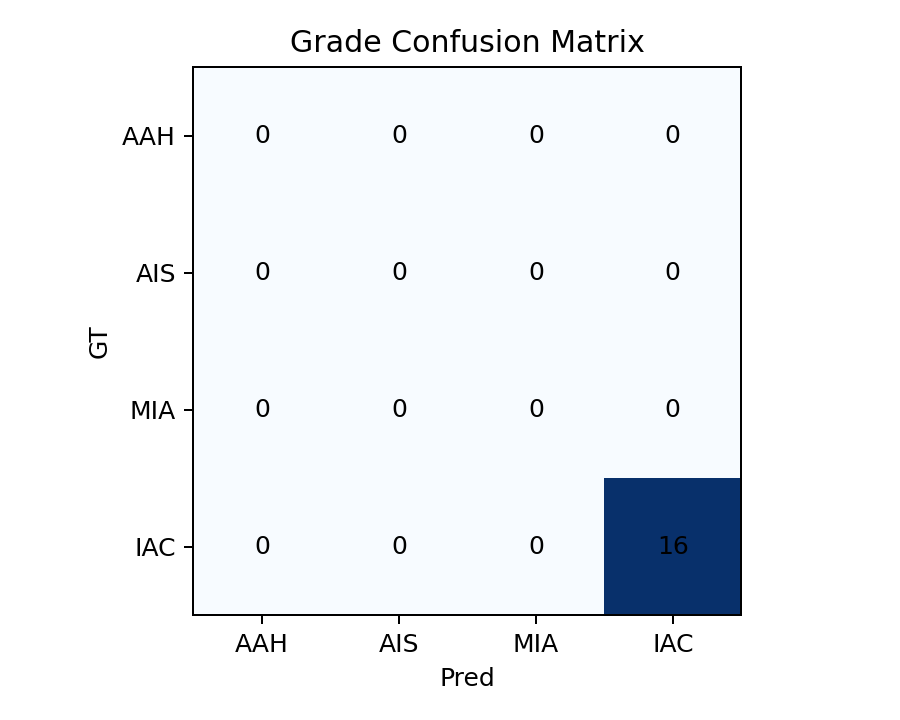
\includegraphics[width=0.75\linewidth]{figures/grade_confusion}
\caption{浸润等级分类混淆矩阵（grade\_confusion）。}
\label{fig:grade-confusion}
\end{figure}

\subsection*{5.4 小结}

上述结果来自单次验证 run，表明：在现有私有数据与设定下，结节勾画与分级分类可达较高成功率；报告四段通过率与幻觉率仍有优化空间，建议结合约束解码与模板检查进一步改进（见 EXPERIMENT\_REPORT.md 中的建议）。训练损失曲线与结构/长度/混淆矩阵图可直接用于方法章节或附录的“实验与结果”部分。
 或直接粘贴本段
% 图表文件：将以下 4 张图放入与主 .tex 同级的 figures/ 目录：
%   - train_loss_curve.png   （训练损失曲线）
%   - length_curve.png       （生成长度 vs 参考长度）
%   - structure_coverage.png  （四段结构覆盖率）
%   - grade_confusion.png    （分类混淆矩阵）
% ============================================================

\section*{五、实验设置与结果（Experiments and Results）}

\subsection*{5.1 实验设置}

\textbf{数据与任务：} 采用私有肺结节 CT 影像-报告配对数据及 pGGN 浸润分级标注（AAH/AIS/MIA/IAC 四分类）；训练阶段使用 Stage~2 联合优化“描述生成 + 分级诊断”，视觉编码保留 28$\times$28 级别高分辨率特征，Mamba-2.8B 作为语言骨干。

\textbf{训练配置：} 最大视觉 token 数 144，最大文本长度 640，batch size 4，学习率 1e-5，epoch 30；梯度裁剪与梯度累积按需启用；日志与 checkpoint 落盘至指定输出目录。

\textbf{验证与评测：} 在 23 例私有验证集上运行端到端推理（报告生成 + 结节勾画 + 分级预测），从 \texttt{meta.json} 与逐样本输出中汇总：报告四段结构通过率、幻觉率、生成长度分布、结节勾画成功率、分类准确率及混淆矩阵。

\subsection*{5.2 主要数值结果}

表~\ref{tab:exp-summary} 给出本次验证 run（run\_20260228\_192037）的汇总指标，供正文引用。

\begin{table}[htbp]
\centering
\footnotesize
\renewcommand{\arraystretch}{1.2}
\begin{tabular}{ll}
\toprule
\textbf{指标} & \textbf{数值} \\
\midrule
验证样本数 & 23 \\
报告四段结构通过率 & 0.00\% \\
幻觉率（规则检测） & 30.43\% \\
生成长度均值 / 中位数 & 215.9 / 210 \\
参考长度均值 / 中位数 & 427.2 / 356 \\
结节勾画成功率 & 100\% \\
分级可评估样本数 & 16 \\
分级分类准确率 & 100\% \\
\bottomrule
\end{tabular}
\caption{私有验证 run\_20260228\_192037 汇总指标（summary.json）。}
\label{tab:exp-summary}
\end{table}

\subsection*{5.3 附图（可直接放汇报/论文）}

\textbf{图~\ref{fig:train-loss}：训练损失曲线。} Stage~2 训练过程中 caption loss 随 step 变化，用于说明收敛情况。

% 插入位置 1：训练损失曲线
\begin{figure}[htbp]
\centering
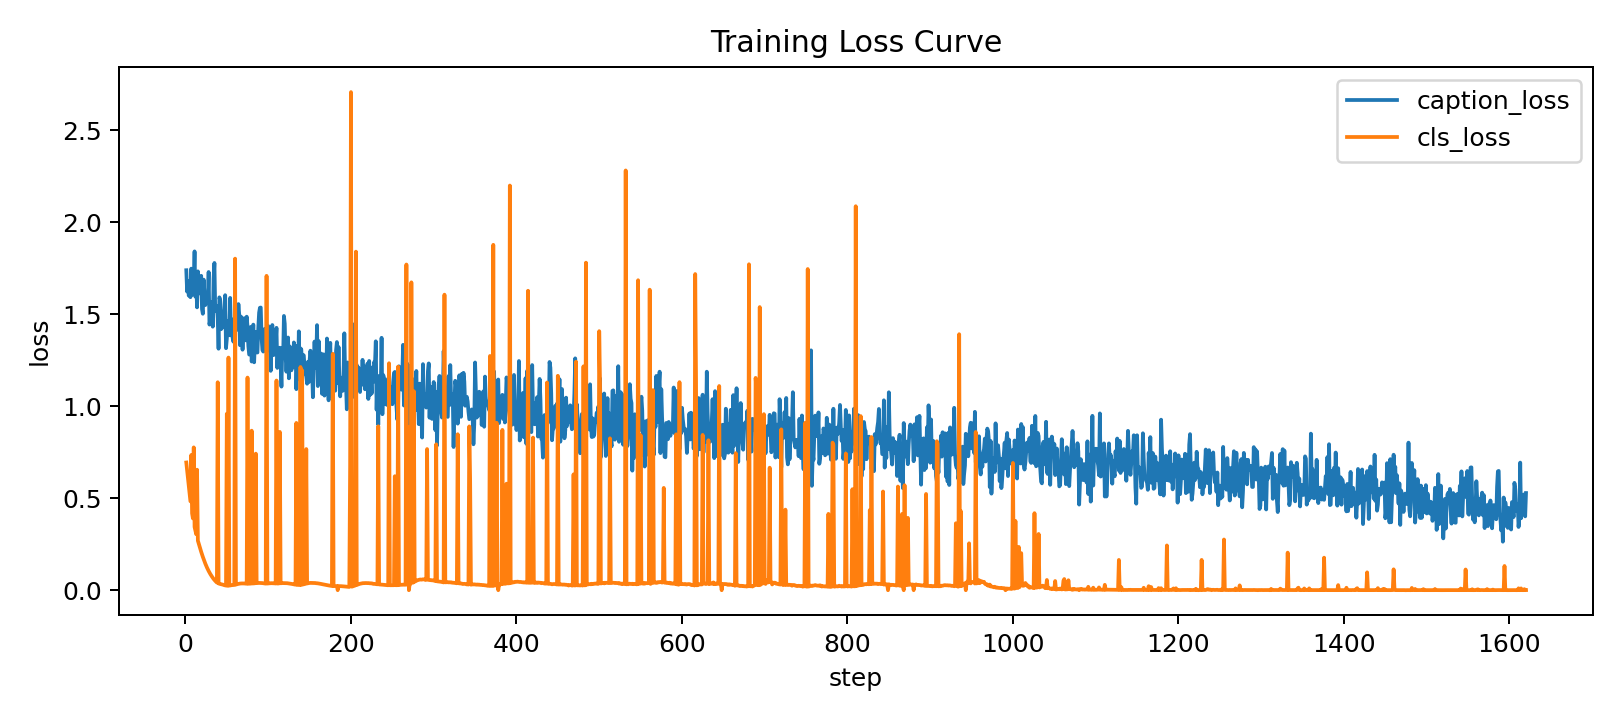
\includegraphics[width=0.85\linewidth]{figures/train_loss_curve}
\caption{Stage~2 训练损失曲线（caption loss vs.\ training step）。}
\label{fig:train-loss}
\end{figure}

\textbf{图~\ref{fig:length-curve}：生成长度 vs.\ 参考长度。} 生成报告 token 长度与参考报告长度的分布对比，用于分析文本长度与截断情况。

% 插入位置 2：生成长度 vs 参考长度
\begin{figure}[htbp]
\centering
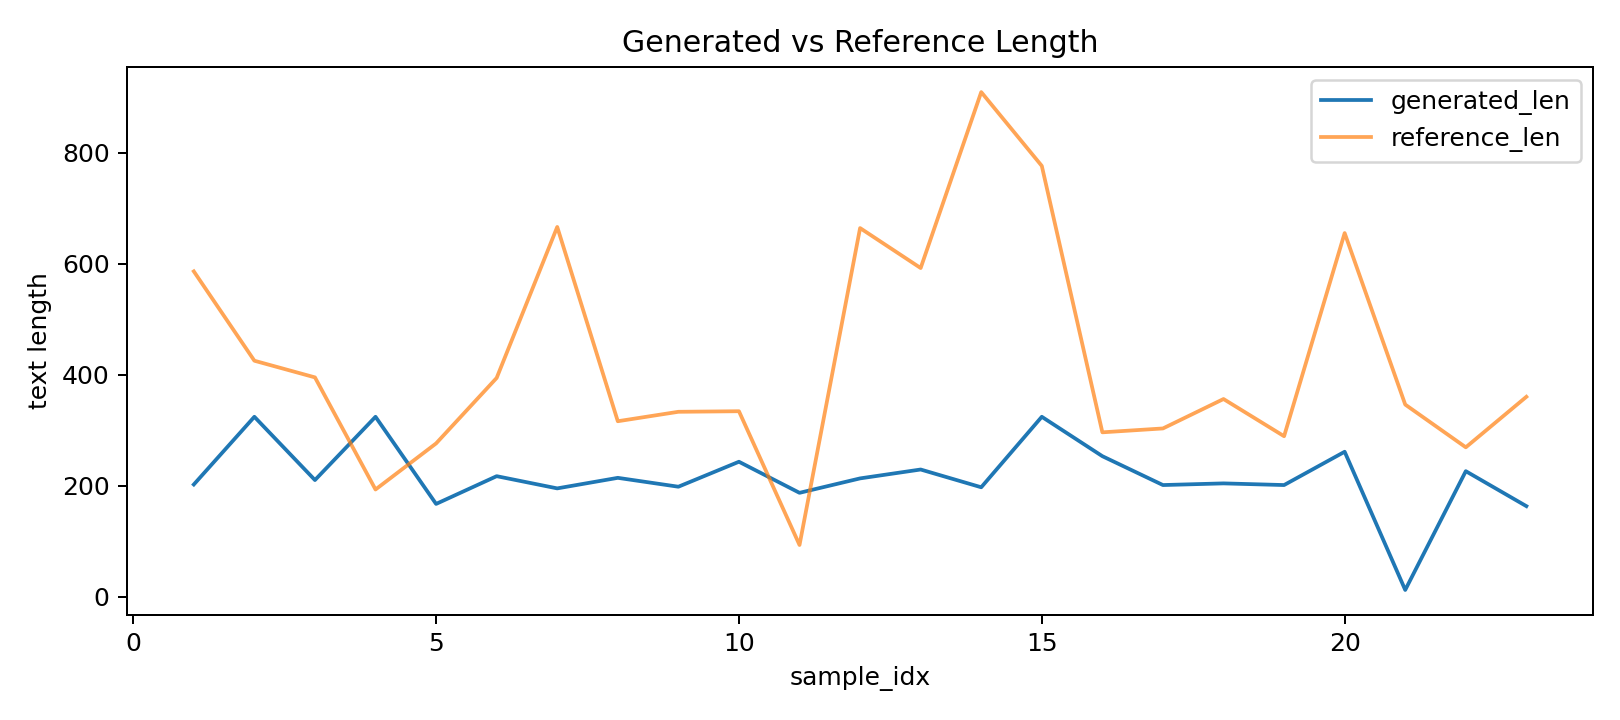
\includegraphics[width=0.85\linewidth]{figures/length_curve}
\caption{生成长度与参考长度分布（length\_curve）。}
\label{fig:length-curve}
\end{figure}

\textbf{图~\ref{fig:structure-coverage}：四段结构覆盖率。} 报告“所见 / 结论 / 建议 / 病理倾向”四段结构的覆盖情况。

% 插入位置 3：四段结构覆盖率
\begin{figure}[htbp]
\centering
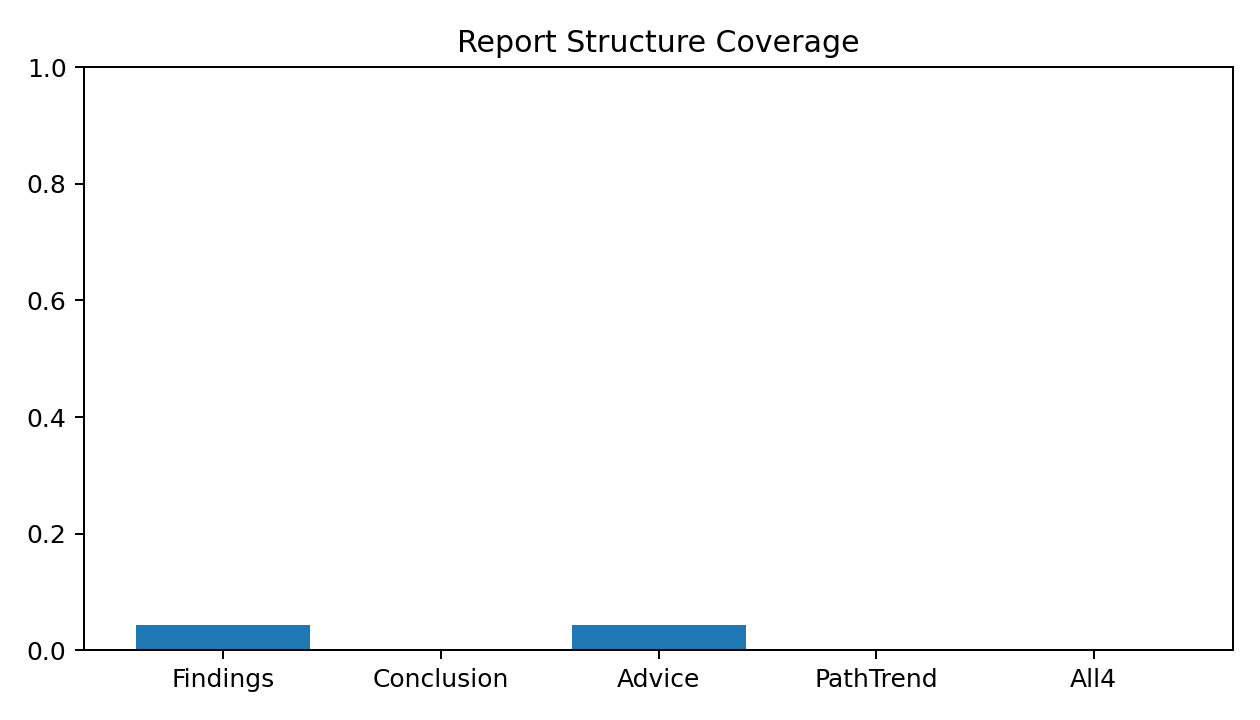
\includegraphics[width=0.85\linewidth]{figures/structure_coverage}
\caption{四段结构覆盖率（structure\_coverage）。}
\label{fig:structure-coverage}
\end{figure}

\textbf{图~\ref{fig:grade-confusion}：分类混淆矩阵。} 浸润等级（AAH/AIS/MIA/IAC）预测与真实标签的混淆矩阵。

% 插入位置 4：分类混淆矩阵
\begin{figure}[htbp]
\centering
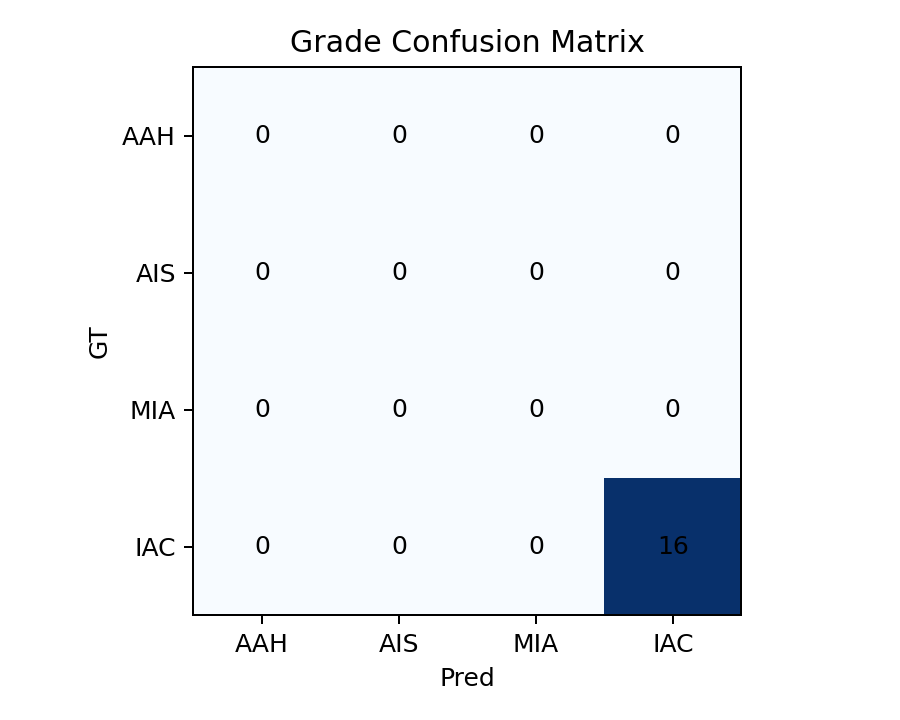
\includegraphics[width=0.75\linewidth]{figures/grade_confusion}
\caption{浸润等级分类混淆矩阵（grade\_confusion）。}
\label{fig:grade-confusion}
\end{figure}

\subsection*{5.4 小结}

上述结果来自单次验证 run，表明：在现有私有数据与设定下，结节勾画与分级分类可达较高成功率；报告四段通过率与幻觉率仍有优化空间，建议结合约束解码与模板检查进一步改进（见 EXPERIMENT\_REPORT.md 中的建议）。训练损失曲线与结构/长度/混淆矩阵图可直接用于方法章节或附录的“实验与结果”部分。
 或直接粘贴本段
% 图表文件：将以下 4 张图放入与主 .tex 同级的 figures/ 目录：
%   - train_loss_curve.png   （训练损失曲线）
%   - length_curve.png       （生成长度 vs 参考长度）
%   - structure_coverage.png  （四段结构覆盖率）
%   - grade_confusion.png    （分类混淆矩阵）
% ============================================================

\section*{五、实验设置与结果（Experiments and Results）}

\subsection*{5.1 实验设置}

\textbf{数据与任务：} 采用私有肺结节 CT 影像-报告配对数据及 pGGN 浸润分级标注（AAH/AIS/MIA/IAC 四分类）；训练阶段使用 Stage~2 联合优化“描述生成 + 分级诊断”，视觉编码保留 28$\times$28 级别高分辨率特征，Mamba-2.8B 作为语言骨干。

\textbf{训练配置：} 最大视觉 token 数 144，最大文本长度 640，batch size 4，学习率 1e-5，epoch 30；梯度裁剪与梯度累积按需启用；日志与 checkpoint 落盘至指定输出目录。

\textbf{验证与评测：} 在 23 例私有验证集上运行端到端推理（报告生成 + 结节勾画 + 分级预测），从 \texttt{meta.json} 与逐样本输出中汇总：报告四段结构通过率、幻觉率、生成长度分布、结节勾画成功率、分类准确率及混淆矩阵。

\subsection*{5.2 主要数值结果}

表~\ref{tab:exp-summary} 给出本次验证 run（run\_20260228\_192037）的汇总指标，供正文引用。

\begin{table}[htbp]
\centering
\footnotesize
\renewcommand{\arraystretch}{1.2}
\begin{tabular}{ll}
\toprule
\textbf{指标} & \textbf{数值} \\
\midrule
验证样本数 & 23 \\
报告四段结构通过率 & 0.00\% \\
幻觉率（规则检测） & 30.43\% \\
生成长度均值 / 中位数 & 215.9 / 210 \\
参考长度均值 / 中位数 & 427.2 / 356 \\
结节勾画成功率 & 100\% \\
分级可评估样本数 & 16 \\
分级分类准确率 & 100\% \\
\bottomrule
\end{tabular}
\caption{私有验证 run\_20260228\_192037 汇总指标（summary.json）。}
\label{tab:exp-summary}
\end{table}

\subsection*{5.3 附图（可直接放汇报/论文）}

\textbf{图~\ref{fig:train-loss}：训练损失曲线。} Stage~2 训练过程中 caption loss 随 step 变化，用于说明收敛情况。

% 插入位置 1：训练损失曲线
\begin{figure}[htbp]
\centering
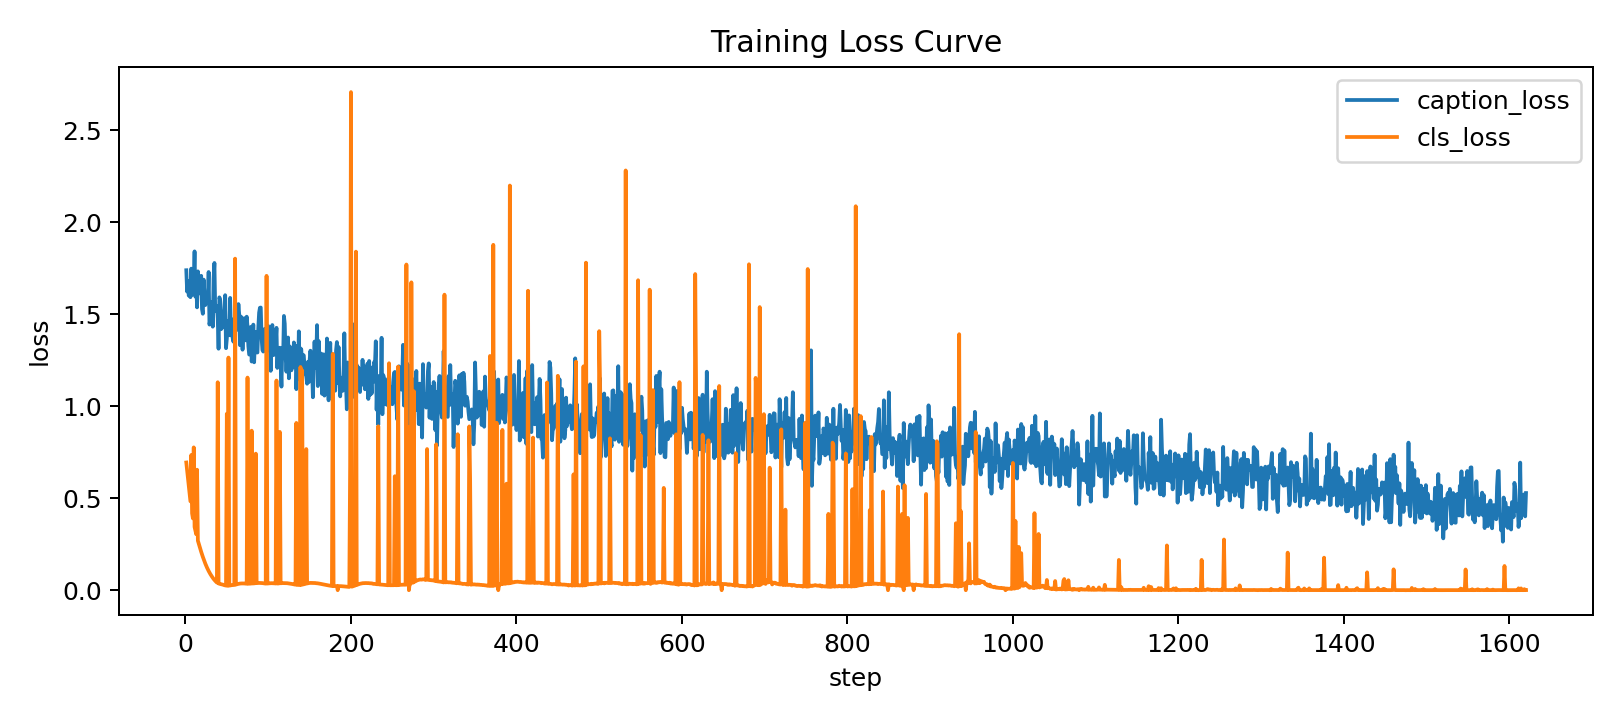
\includegraphics[width=0.85\linewidth]{figures/train_loss_curve}
\caption{Stage~2 训练损失曲线（caption loss vs.\ training step）。}
\label{fig:train-loss}
\end{figure}

\textbf{图~\ref{fig:length-curve}：生成长度 vs.\ 参考长度。} 生成报告 token 长度与参考报告长度的分布对比，用于分析文本长度与截断情况。

% 插入位置 2：生成长度 vs 参考长度
\begin{figure}[htbp]
\centering
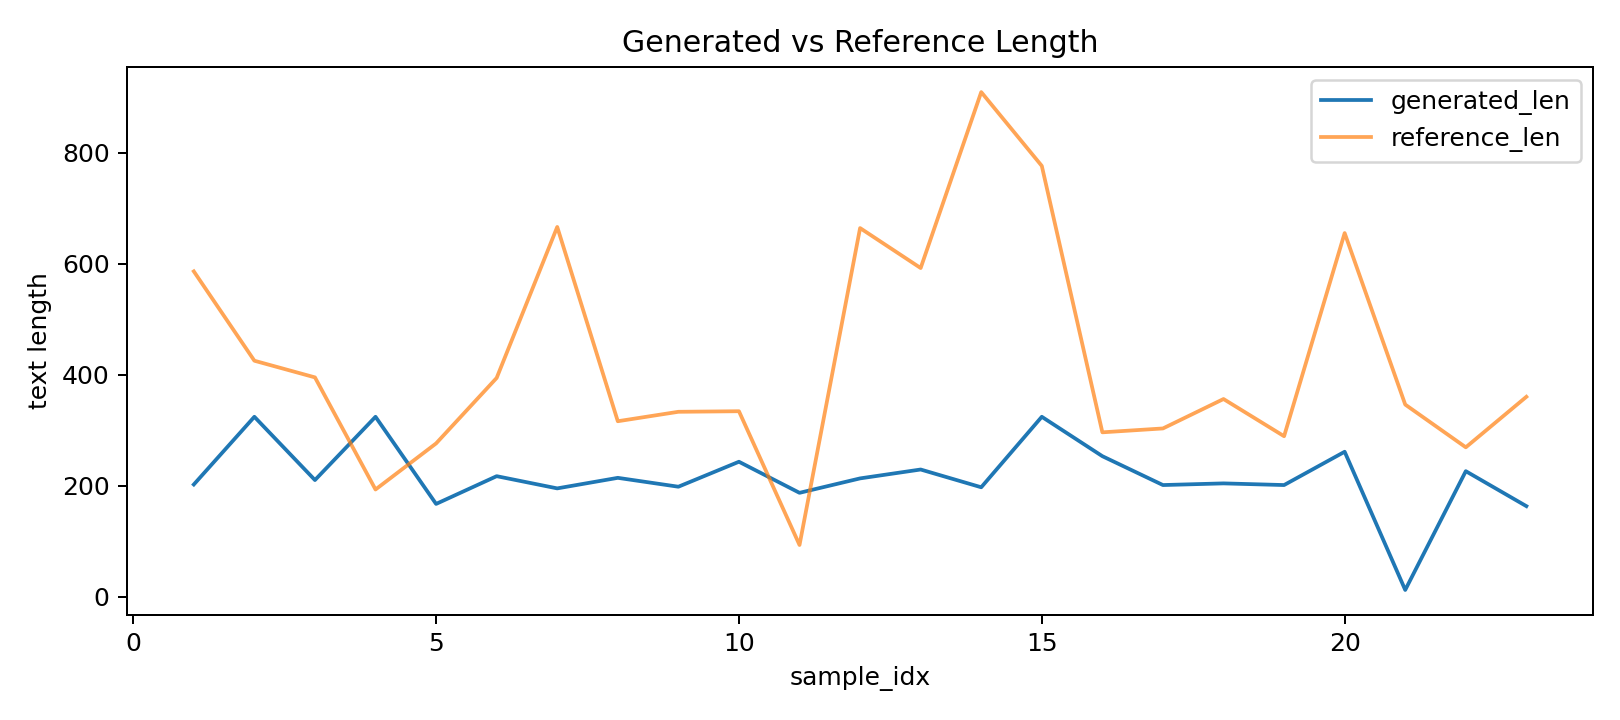
\includegraphics[width=0.85\linewidth]{figures/length_curve}
\caption{生成长度与参考长度分布（length\_curve）。}
\label{fig:length-curve}
\end{figure}

\textbf{图~\ref{fig:structure-coverage}：四段结构覆盖率。} 报告“所见 / 结论 / 建议 / 病理倾向”四段结构的覆盖情况。

% 插入位置 3：四段结构覆盖率
\begin{figure}[htbp]
\centering
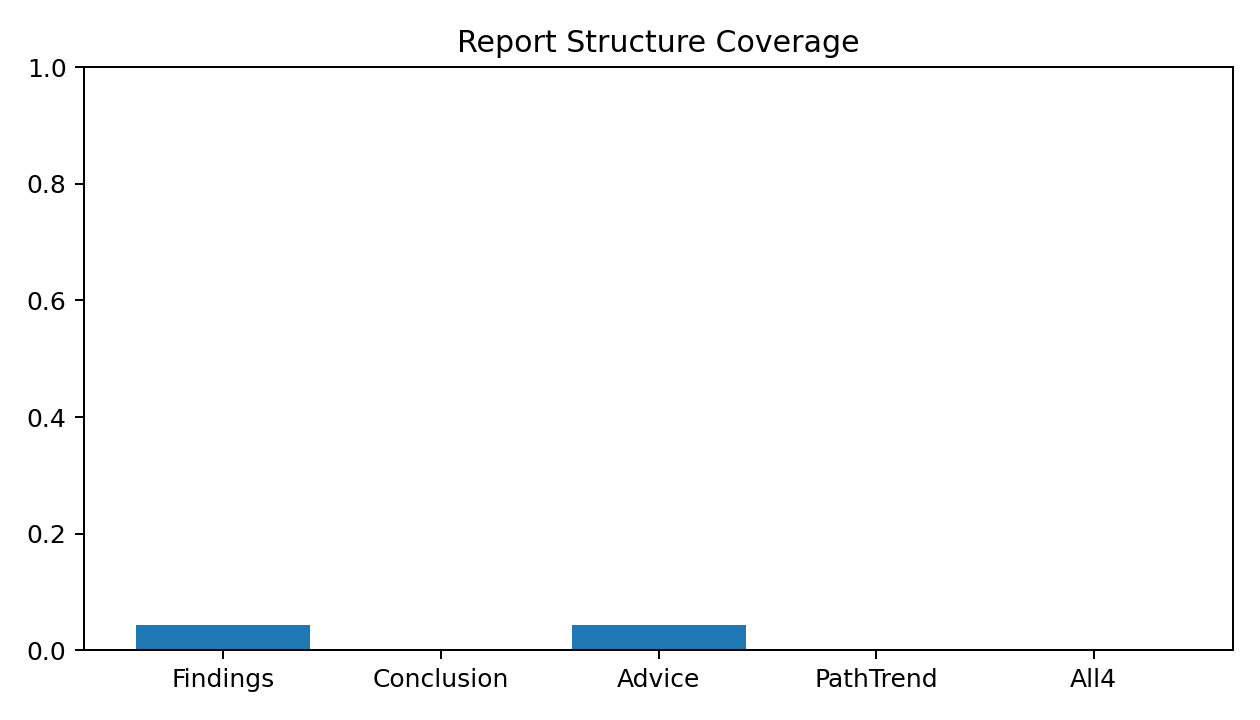
\includegraphics[width=0.85\linewidth]{figures/structure_coverage}
\caption{四段结构覆盖率（structure\_coverage）。}
\label{fig:structure-coverage}
\end{figure}

\textbf{图~\ref{fig:grade-confusion}：分类混淆矩阵。} 浸润等级（AAH/AIS/MIA/IAC）预测与真实标签的混淆矩阵。

% 插入位置 4：分类混淆矩阵
\begin{figure}[htbp]
\centering
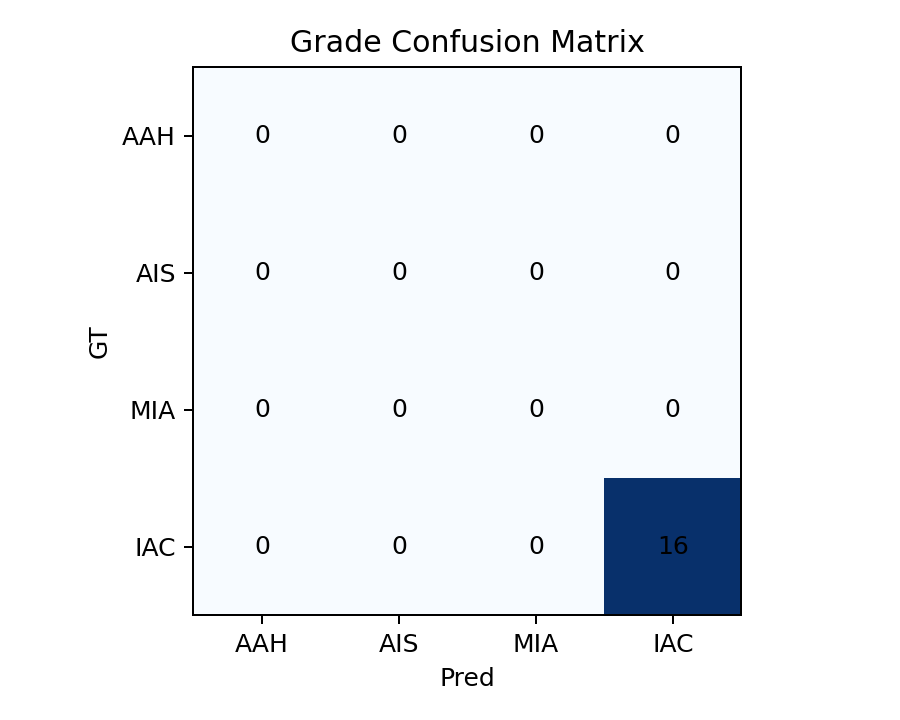
\includegraphics[width=0.75\linewidth]{figures/grade_confusion}
\caption{浸润等级分类混淆矩阵（grade\_confusion）。}
\label{fig:grade-confusion}
\end{figure}

\subsection*{5.4 小结}

上述结果来自单次验证 run，表明：在现有私有数据与设定下，结节勾画与分级分类可达较高成功率；报告四段通过率与幻觉率仍有优化空间，建议结合约束解码与模板检查进一步改进（见 EXPERIMENT\_REPORT.md 中的建议）。训练损失曲线与结构/长度/混淆矩阵图可直接用于方法章节或附录的“实验与结果”部分。

% ========== 若 \input 报错，请将 paper_section_experiments.tex 的正文全部粘贴到此处 ==========

\end{document}
